% 编译使用xelatex
\documentclass{ctexart}

\usepackage{amsmath}
\usepackage{amsfonts}
\usepackage{amssymb}
\usepackage{tabularx}
\usepackage{bigfoot}
\usepackage{fancyvrb}
\usepackage{graphicx}
\usepackage{subfig}
\usepackage{placeins}       % \FloatBarrier
% define new stretchable column types
\newcolumntype{L}{>{\raggedright\arraybackslash}X}
\newcolumntype{R}{>{\raggedleft\arraybackslash}X}
\newcolumntype{C}{>{\centering\arraybackslash}X}

\DeclareMathOperator{\Def}{\;\mathbf{Def}\;}
\DeclareMathOperator{\Ref}{\;\mathbf{Ref}\;}

% for simulating booktabs rules; so they work with vertical lines
\newlength{\Oldarrayrulewidth}
\newcommand{\Cline}[2]{
  \noalign{\global\setlength{\Oldarrayrulewidth}{\arrayrulewidth}}
  \noalign{\global\setlength{\arrayrulewidth}{#1}}\cline{#2}
  \noalign{\global\setlength{\arrayrulewidth}{\Oldarrayrulewidth}}}
\newcommand{\Hline}[1]{
  \noalign{\global\setlength{\Oldarrayrulewidth}{\arrayrulewidth}}
  \noalign{\global\setlength{\arrayrulewidth}{#1}}\hline
  \noalign{\global\setlength{\arrayrulewidth}{\Oldarrayrulewidth}}}
\newcommand{\Topline}{\Hline{0.08em}}
\newcommand{\Bottomline}{\Hline{0.08em}}
\newcommand{\Midline}{\Hline{0.05em}}
\newcommand{\CMidLine}[1]{\Cline{0.05em}{#1}}


\title{编译原理}

\begin{document}
\maketitle

\tableofcontents

\section{词法分析}
\paragraph{目的}
    将字符流转为符号流.
\paragraph{符号定义} \begin{itemize}
        \item 巴克斯范式
        \item 正则表达式
        \item 混合 (如lex的实现)
    \end{itemize}
\paragraph{解析方式}
    基本通过正则表达式语言和有限状态自动机的等价原理, 将符号定义转为正则表达式,
    之后变为有限状态自动机, $\epsilon$-NFA到NFA到DFA.\par
    通常采取最长匹配方法, 即允许自动机向前偷看一个符号.
    如果当前满足一个符号, 但是按照偷看符号转移后不满足任何符号, 则返回当前匹配的符号.

\section{语法分析}
\paragraph{目的}
    将符号串解析为符合程序语法的生成树
\paragraph{语法描述}
    通过上下文无关语言描述语法. 后记此语法为$G[S]$
\paragraph{惯例} \begin{itemize}
        \item 终结符串最后还认为有一个终止符号$\$$ (课程中是$\#$)
        \item $\alpha, \beta \ldots \in (V\cup T)^*$
        \item $w \in T^*$
        \item $a, b \ldots \in T$
        \item $A, B \ldots \in V$
        \item $X, Y \ldots \in V\cup T$
    \end{itemize}
\subsection{自顶向下分析}
    从起始符号$S$开始, 不断利用产生式展开非终结符, 直到原串.\par
\paragraph{不确定性} 这样的方法有两个不确定性 \begin{enumerate}
        \item 选择哪一个非终结符展开
        \item 选择哪一个产生式
    \end{enumerate}\par
    第一个问题很容易, 每次都选择当前符号串$w A \alpha$的最左边的非终结符$A$展开.
\subsubsection{产生式的选择}
\paragraph{向前查看} 对于$wA\alpha$, 选择产生式如果只考虑$A$, 则没有任何线索, 能够确定选择哪一个产生式.\par
    设$\alpha = X_1 X_2 \ldots X_l$.
    由上, 选择产生式时,
    不仅考虑$A$, 还考虑$X_1, X_2 \ldots X_k,\; (k < l)$,
    选择的产生式$p$是它们的函数$p = f(A, X_1 \ldots X_k)$.\par
    称这种方法为LL(k)方法. 下述LL(1)方法.
\paragraph{First函数} First是符号串的函数, 定义如下\[
    First(\alpha) = \{a \in T \;|\; \exists \beta\,:\,\alpha \Rightarrow^* a\beta\}\]
    特别地, 如果$\alpha \Rightarrow^* \epsilon$, 则说$\epsilon \in First(\alpha)$.
    意义是符号串对应的终结符串的首个终结符的取值集合.
\paragraph{Follow函数} Follow是非终结符的函数, 定义如下\[
    Follow(A) = \{a \in T \;|\; \exists \alpha, \beta \,:\, S\$ \Rightarrow^* \alpha A \beta\$, a \in First(\beta\$)\}
    \]
    意思是$G[S]$句型中中, 可能跟在$A$的后面的终结符所有取值.
\paragraph{选择产生式} 希望展开$A$, 并且$\text{lookahead} = a$, 则选择的产生式$A \to \beta$应当满足\[
    a \in PS(A \to \beta) = \begin{cases}
        First(\beta) & \epsilon \not\in First(\beta)\\
        First(\beta) \cup Follow(A) - \{\epsilon\} & \epsilon \in First(\beta)
    \end{cases} \]
    如果$\forall A \in V, a \in T$有$\Big|\{A \to \beta \;|\; a \in PS(A \to \beta)\}\Big| = 1$ (即产生式的选择唯一),
    则称$G[S]$是LL(1)文法, 可以按照上述方法解析.
\subsubsection{First和Follow的计算}
\paragraph{First的计算} 考虑计算$First(\alpha)$, 设$\alpha = X_1 X_2 \ldots X_k$.\par
    若$X_1\ldots X_{l-1}$可空, $X_l$不可空 (显然终结符不可空), 有\[
        First(\alpha) = \cup_{1 \le i \le l} \left( First(X_i) - \{\epsilon\} \right) \]\par
    若$X_1 \ldots X_k$都可空, 则\[
        First(\alpha) = \cup_{1 \le i \le k} First(X_i)\]\par
    非终结符$First(A) = \cup_{\beta\;:\; A \to \beta} First(\beta)$.\par
    通过迭代即可求解如上的集合约束问题.
\paragraph{Follow的计算} 考虑计算$Follow(A)$. 首先寻找所有形如$B \to \alpha A \beta$的产生式.\par
    如果$\epsilon \not\in First(\beta)$, 则$Follow(A) \supseteq First(\beta)$.\par
    如果$\epsilon \in First(\beta)$, 则$Follow(A) \supseteq First(\beta) \cup Follow(B) - \{\epsilon\}$.\par
    通过迭代求解如上的集合约束问题, 要求$Follow(A)$取最小 (即满足上述条件的最小集合).
\subsubsection{递归下降程序} 每个非终结符的解析都是一个函数.
    其中根据lookahead选择产生式, 匹配非终结符就调用对应函数, 匹配非终结符就直接\texttt{match\_token}.\par
    常见的递归下降程序如\begin{verbatim}
    void parse_B()
    {
        switch (lookahead) {
            case c: 
                // B -> c A d,      First(c A d) = {c}
                match_token(c); 
                parse_A()
                match_token(d);
                break;
            case b: 
                // B -> epsilon,    Follow(B) = {b}
                break;
            default:
                // no production matches here
                report error;
        }
    }\end{verbatim}
\subsubsection{表驱动程序}
    记$M[A, a]$表示希望展开$A$, $\text{lookahead} = a$时, 按照上述方法得到的可用产生式.\par
    表驱动利用一个栈, 最初栈中只有$S\$$, $S$在栈顶. 之后重复检查栈顶$X$和输入$\text{lookahead} = a$ \begin{itemize}
        \item $X = \$$, 分析完成
        \item $X \in T$, 此时应有$X$等于$a$. 符合则消耗$a$, 否则报错
        \item $X \in V$, 设$M[X, a] = X \to \alpha$, 则$X$出栈, $\alpha$从右到左入栈
    \end{itemize}
\subsubsection{语法变换}
    通过消除左递归和公共左公因子, 能将很多非LL(1)语言转换为LL(1)语言, 如$S \to Sa | b$.
\paragraph{去除直接左递归} 原为\begin{align*}
        A & \to A \alpha_1 \,|\, A \alpha_2 \,|\, \ldots \,|\, \beta_1 \,|\, \beta_2 \,|\, \ldots
    \end{align*}改写为\begin{align*}
        A &\to \beta_1 B \,|\, \beta_2 B \,|\, \ldots \\
        B &\to \alpha_1 B \,|\, \alpha_2 B \,|\, \ldots \,|\, \epsilon
    \end{align*}
\paragraph{去除间接左递归} 要求原文法无环$A \not\Rightarrow^+ A$, 无$\epsilon$产生式$A \to \epsilon$.\par
    首先将非终结符编号为$A_1, A_2 \ldots A_n$, 然后\begin{verbatim} 
for i = 1 to n
    for j = 1 to i-1
        对于所有 A_i -> A_j \alpha,
            代替以 A_i -> \beta \alpha,
            其中 A_j -> \beta
    消除A_i的直接递归
\end{verbatim}
\paragraph{消除左公因子} 直接将左公因子作为新的符号即可.
\subsection{Bottom-up parsing}
    从输入串开始, 不停将串中一个子串规约成一个非终结符, 直到规约成$S$.
\paragraph{不确定性} 有2个不确定性
    \begin{enumerate}
        \item 选择哪个子串
        \item 选择哪个产生式, 如果有多个产生式的右边一样
    \end{enumerate}
    采用一类称为LR分析的解决此问题.
    每次都选择``句柄'', 选择的产生式通过LR分析表确定.
\subsubsection{概念}
    以下是语法本身的概念
    \begin{description}
        \item[短语] 如果$S\Rightarrow^* \alpha A \beta$且$A \Rightarrow^+ \gamma$,
                则称$\gamma$是$\alpha A \beta$中$A$的短语.\\
                在$\alpha A \beta$确定的情况下, 可以称$\gamma$是$A$的短语.
                这时在$S \Rightarrow^* \alpha \gamma \beta$的分析树中,
                $\gamma$是$A$的子树的叶遍历, 并且要求$A$本身不能是叶子.
        \item[直接短语] $S\Rightarrow^* \alpha A \beta$且$A \Rightarrow \gamma$,
                则称$\gamma$是$\alpha A \beta$中$A$的直接短语.\\
                直接短语就是可以一步推出的短语.
                在$\alpha \gamma \beta$的分析树中, 对应的是$A$所有儿子都是叶子的情况.
        \item[句柄] $S \Rightarrow^* \alpha A w$且$A \Rightarrow \beta$,
                则称$\beta$是$\alpha A w$中$A$的句柄.\par
                句柄就是从左到右第一个出现的直接短语.
                可以理解为``最右推导''反过来就是``最左规约''.
    \end{description}
\subsubsection{通用框架}
    所有LR分析, 分析框架是一样的, 只有分析表是不一样的.\par
    基本分析方法就是基于一个栈, 从左到右扫描输入串,
    每次根据当前控制状态, 栈中内容 (不限于栈顶), 下一个输入符号来决定动作, 并且转移到新的控制状态.\par
    所有LR分析都有一个$action[i, a]$表
        \[\begin{array}{ll}
            \Topline
            action[i, a] & \text{含义}\\
            \Midline
            \text{shift}\,j & \text{将}a\text{移入栈中, 状态变为}j \\
            \text{reduce}\,A\to\alpha & \text{此时栈顶应为}\alpha\text{, 规约栈顶. 之后}A\text{入栈, 状态变为}goto[i, A] \\
            \text{success} & \text{分析成功, 即将原输入串规约成了}S \\
            \text{error} & \text{出错} \\
            \Bottomline
        \end{array}\]\par
    所有LR分析都有一个$goto[i, A]$表.
    $goto[i, A] = j$表示当前状态为$i$,
    一个非终结符$A$入栈后, 那么状态变为$j$.\par
    所有LR分析都是用增广文法, 即加入产生式 $S' \to S$的文法$G[S']$. $S' \to .S$对应的状态为初状态.

\subsubsection{LR(0)分析表}
\paragraph{item} 加点的产生式. 为了方便认识用方括号括起.
\paragraph{closure} 考虑item间的关系$R$, 为$[A \to \alpha . B \beta] \;R\; [B \to .\gamma]$.
    定义$closure(I)$等于$I$在关系$R$的传递闭包, $I$是item集合.
\paragraph{go} $I \text{ is closure},\;X \in V \cup T$\[
    go(I, X) = closure(\{[A \to \alpha X .\beta] \;|\; [A \to \alpha . X \beta] \in I\})\]
\paragraph{action} \[action[i, a] = \begin{cases}
    \text{shift}\; j          & J = go(I, a)\\
    \text{reduce}\; A\to\beta & [A \to \beta.] \in I\\
    \text{accept}             & [S' \to S.] \in I\\
    \text{error}              & \text{otherwise}
    \end{cases}\]
\paragraph{goto} \[goto[i, A] = j \quad J = go(I, A)\]

\subsubsection{SLR(1)分析表}
    基本同LR(0), 但是完成reduce的条件变得更精确.\par
    原理: 完成规约$A\to\alpha$时, 下一个输入$a$应当满足$a \in Follow(A)$.
\paragraph{action} \[action[i, a] = \begin{cases}
    \text{shift}\; j          & J = go(I, a)\\
    \text{reduce}\; A\to\beta & [A \to \beta.] \in I \land a \in Follow(A)\\
    \text{accept}             & [S' \to S.] \in I\\
    \text{error}              & \text{otherwise}
    \end{cases}\]

\subsubsection{LR(1)分析表}
\paragraph{item} 之前是一遇到可规约的$A \to \alpha.$就规约 (规则2.),
    但是不一定是这样 (前看$\alpha$之后一个符号得到的信息被忽略了).\par
    item的表示是$[A \to \alpha . \beta, a],\quad a \in T$. 如果$\beta \neq \epsilon$, 那么一切和SLR一样.\par
    如果$\beta = \epsilon$, 那么当且仅当$a \in Follow(A)$时, 才进行规约.
\paragraph{closure} $[A \to \alpha . B \beta, a]  \; \mathbf{R} \;  [B \to .\gamma, b] \quad b \in \mathbf{FIRST}(\beta a)$
    如上关系的闭包.
\paragraph{构造go} $go(I, X) = closure([A \to \alpha X. \beta] \,|\, [A \to \alpha . X \beta] \in I)$
\paragraph{构造item集} 从$closure([S' \to .S, \$])$按照$go$拓展得图.
\paragraph{初态} $I_0 = closure(\{[S' \to .S,\, \$]\})$
\paragraph{action} 更精确的描述了完成reduce的条件
%    原理: 完成规约$A\to\alpha$时, 下一个输入$a$应当满足$a \in Follow(A\to\alpha)$,
%        即各个产生式之后能跟的符号是不同的. 如$S \to Ab;\quad A \to Aa\;|\;\epsilon$.
%        产生式$A\to Aa$之后只能跟$b$, 
%
%$
%S ::= A a | b A c | d c | b d a
%
%A ::= d
%$
% TODO
    \[ action[I, a] = \begin{cases}
        \text{shift}\; go(I, a)    & [A \to \alpha .a \beta,\, b] \in I\\
        \text{reduce}\; A\to\alpha & [A \to \alpha.,\, a] \in I,\, A\to\alpha \neq S'\to S\\
        \text{accept}              & [S' \to S., \$] \in I\\
        \text{error}               & \text{otherwise}\end{cases} \]

\subsubsection{LALR(1)}
    和LR(0)一样状态数目.
    其余方法和LR(1)相同.
\paragraph{合并LR(1)同芯状态} 同芯: $[A\to\alpha.\beta, a]$中$A\to\alpha.\beta$相同


\section{符号表}
\paragraph{基本概念}
    不同的作用域有自己的符号表, 某处可见的符号是其自身包含所有父亲作用域 (亦称开作用域) 符号表的并.
\paragraph{实现} 可以实现为全局的一个符号表, 也可以实现成各个作用域符号表的栈.

\section{基于语法的语义计算}
\subsection{基于属性文法}
\subsubsection{基本概念}
\paragraph{定义}
    在CFG基础上, 对每个$X \in V \cup T$关联属性, 记为$X.a, X.b$等.\par
    每个产生式$A\to X_1 X_2 \ldots X_N,\; X_i \in V \cup T, X_0 = A$关联一个语法动作,
    语法动作是若干个属性计算的序列, 每个属性计算形如$X_i.a = f(X_j.b \;|\; j \neq i, b\text{是}X_j\text{的属性}),\; 0 \le m \le N$.
\paragraph{综合属性} $A \to X_0 \ldots X_N$关联的语法动作是$A.a = f(X_i.b)$则称$A.a$是综合属性.
    综合属性代表语法树中自下而上传递的信息.
\paragraph{继承属性} $A \to X_0 \ldots X_N$关联的语法动作是$X_i.a = f(X_j.b),X_i \neq A$则称$X_i.a$是继承属性.
    继承属性代表语法树中自上而下传递的信息.
\paragraph{S-属性文法} 只包含综合属性的属性文法称S-属性文法.
\paragraph{L-属性文法} 允许综合属性和继承属性, 但是语法动作要求有$X_i.a = f(X_{\neq i}.b) =f(X_{< i}.b)$.
    即产生式中某符号的属性不能依赖产生式中位于它之后的符号的属性.

\subsubsection{两趟方法的属性计算}
    生成语法树之后, 计算属性的大致步骤如下
    \begin{enumerate}
        \item 分析语法书中结点属性 (即符号属性) 的依赖关系
        \item 如果依赖关系不存在环, 则按照依赖关系的拓扑顺序计算属性值.\\
        如果依赖关系有环, 认为属性语法不是良定义的, 不予处理.\par
    \end{enumerate}
    两趟方法通用, 但是效率开销较大.

\subsubsection{一趟方法的属性计算}
\paragraph{S-属性文法} 采用自底向上文法分析 (如LR), 每次按$A \to X_1 X_2 \ldots X_N$进行规约时, 一定有$X_1, X_2 \ldots X_N$是栈顶$N$个元素.
    因此将元素属性一并存放在栈中, 每次规约时直接通过栈顶元素$N$个元素$X_1, X_2\ldots X_N$的属性计算$A.a$即可.
\paragraph{L-属性文法} \label{onepass-l-attr-grammar} 采用自顶向下文法分析 (如LL(1)递归下降),
    将继承属性作为参数传入子符号的分析过程, 并且要求子符号分析过程返回子符号的综合属性.\par
    即将$\mathbf{Parse}(A) \to \mathtt{void}$改为$\mathbf{Parse}(A, A.a_I) \to A.a_S$, 其中$A.a_I$表示$A$的继承属性, $A.a_S$表示$A$的综合属性.

\subsection{基于翻译模式}
\subsubsection{基本概念}
\paragraph{翻译模式} 类似属性文法, 但是允许语法动作出现在产生式中任何地方, 表示匹配到该处时即刻执行该语法动作.
\paragraph{消除左递归} 讨论消除左递归时, 保持翻译动作等价. 以直接左递归为例\begin{align*}
        A & \to A_1 \alpha \; \{ A.s = f(A_1.s, \alpha.s)\}\\
        A & \to \beta  \;     \{ A.s = g(\beta.s)\}
    \end{align*}
    按照消除直接左递归的方法变换之后, 变为 \begin{align*}
        A & \to \beta \;     \{ R.i = g(\beta.s) \} \; R \;             \{A.a = f(R.s)\}\\
        R & \to \epsilon  \; \{ R.s = R.i\}\\
        R & \to \alpha \;    \{ R_1.i = f(R.i, \alpha.s) \}\; R_1  \;   \{ R.s = R_1.s \}
    \end{align*}
    可以认为$R.i$中保存了原来式子中所有其左便的所有信息.
\subsubsection{自上而下计算}
    类似\ref{onepass-l-attr-grammar}, 但是计算属性在$\mathbf{parse(A)}$过程中进行.
\subsubsection{自下而上计算}
    使用从下而上分析方法, 将综合属性和符号一起存储在栈中.
    这样有一个问题, 无法访问继承属性, 因为需要在确定非终结符前完成语法动作.
    因此需要提供一种方法实现继承属性的访问.\par
    可以将语法稍作变换, 添加若干空非终结符,
    由它们完成中间的语法规则的计算, 
    使得产生式中间只有复写规则$X_i.i = X_{i-1}.s$.\par
    这样可以沿着复写规则, 对于继承属性$X_i.i$,
    最终找到综合属性$X_j.s$,
    满足$j<i$而且两者是相等的 (根据复写规则).
    这时因为$j < i$, 所以执行$X_i$的分析时$X_j$一定在栈中.
    \begin{figure}%
        \centering
        \subfloat[最初的翻译模式]{{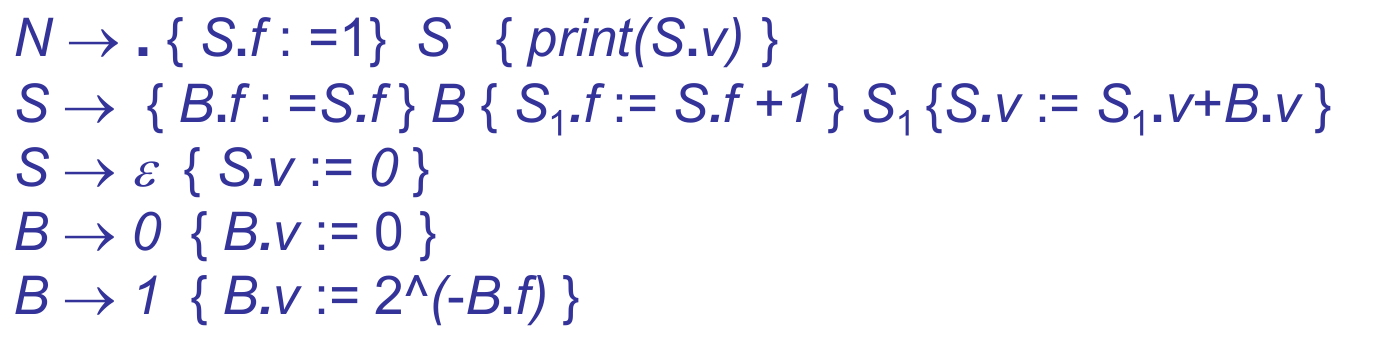
\includegraphics[width=0.95\textwidth]{trans-ex-1.png}}}%
        \\
        \subfloat[转换为适合自下而上的翻译模式]{{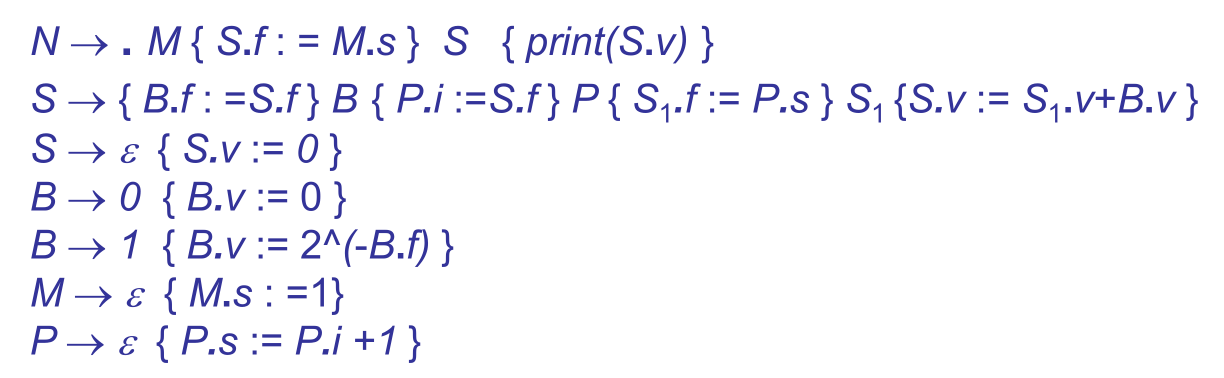
\includegraphics[width=0.95\textwidth]{trans-ex-2.png}}}%
        \\
        \subfloat[规约时代码片段]{{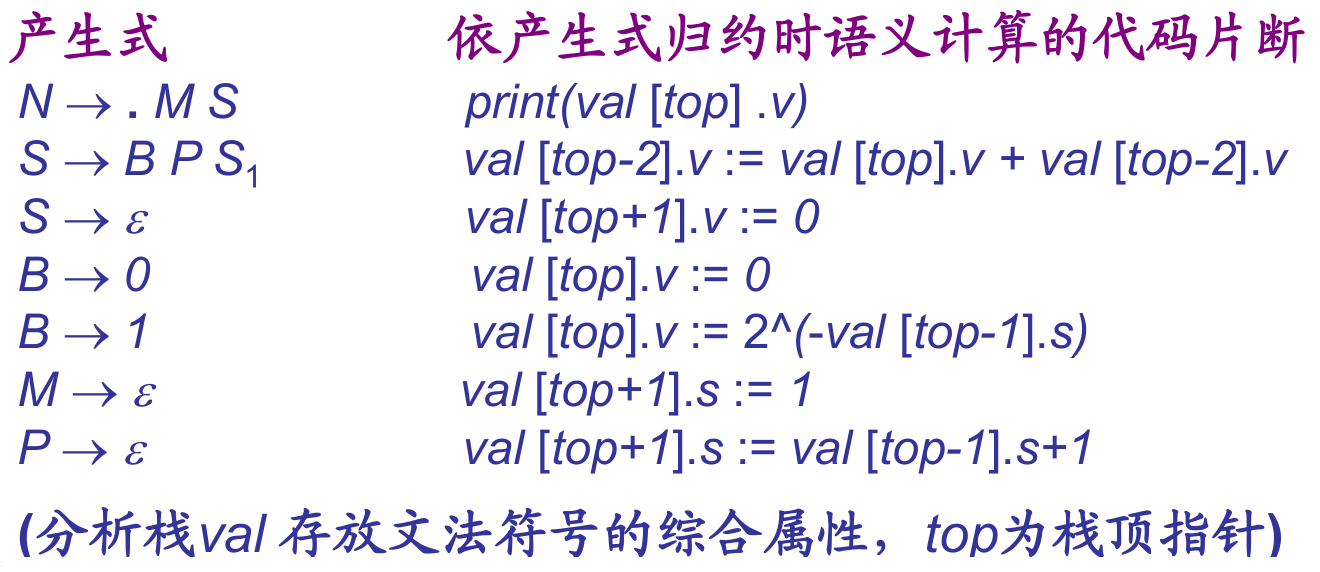
\includegraphics[width=0.95\textwidth]{trans-ex-3.png}}}%
        \caption{自下而上计算的例子}%
    \end{figure}
    \FloatBarrier

\section{中间代码生成}
\subsection{静态语义分析}
    包含类型检查, 作用域分析, 控制流检查等. 通过翻译模式实现.
\subsection{中间代码生成}
    课程中只考虑三地址码的生成.
\subsubsection{布尔表达式的翻译}
\paragraph{直接翻译} 不处理短路特性. 相当于普通表达式的计算.
\paragraph{L-属性文法}
    每个表达式$E$有继承属性$E.true$和$E.false$, 这些属性分别都是标号. 具体如图.
    实现如图\ref{bool-1}
    \begin{figure*}[ht]
    \centering
    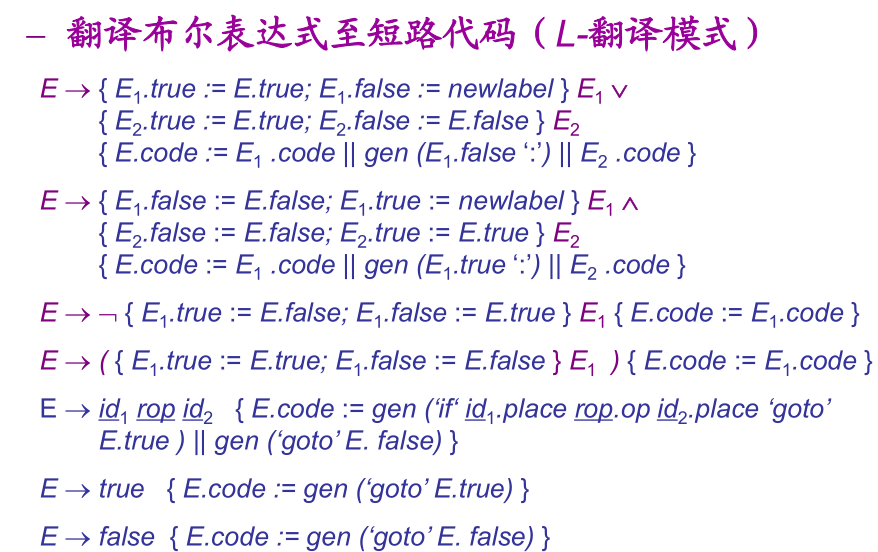
\includegraphics[width=0.9\textwidth]{bool-1.png}
    \caption{L-属性文法的布尔短路翻译}
    \label{bool-1}
    \end{figure*}
    如果翻译循环等, 还需要加入$S.next$等.
\paragraph{S-属性文法}
    将标号作为综合属性, 待顶层布尔表达式翻译完后,
    将所有下层表达式中未知的标号回填. 称为拉链方法 (backpatching).\par
    表达式$E$有两种综合属性$E.truelist$和$E.falselist$,
    包含未确定的, 但是知道是跳转到真还是假的标号.\par
    还包含函数
    \begin{table}[ht!]
        \centering
        \begin{tabularx}{\textwidth}{cL}
            \Topline
            函数名 & 行为\\
            \Midline
            $makelist(initial\_entry)\;\to list$ & 创建一个待回填的表\\
            $merge(list, list)\;\to list$ & 返回两个表的合并\\
            $backpatch(list, lbl)$ & 确定$list$中的标号为$lbl$\\
            \Bottomline
        \end{tabularx}
        \caption{拉链方法的函数}
    \end{table}
    实现如图\ref{bool-2}
    \begin{figure*}[ht]
    \centering
    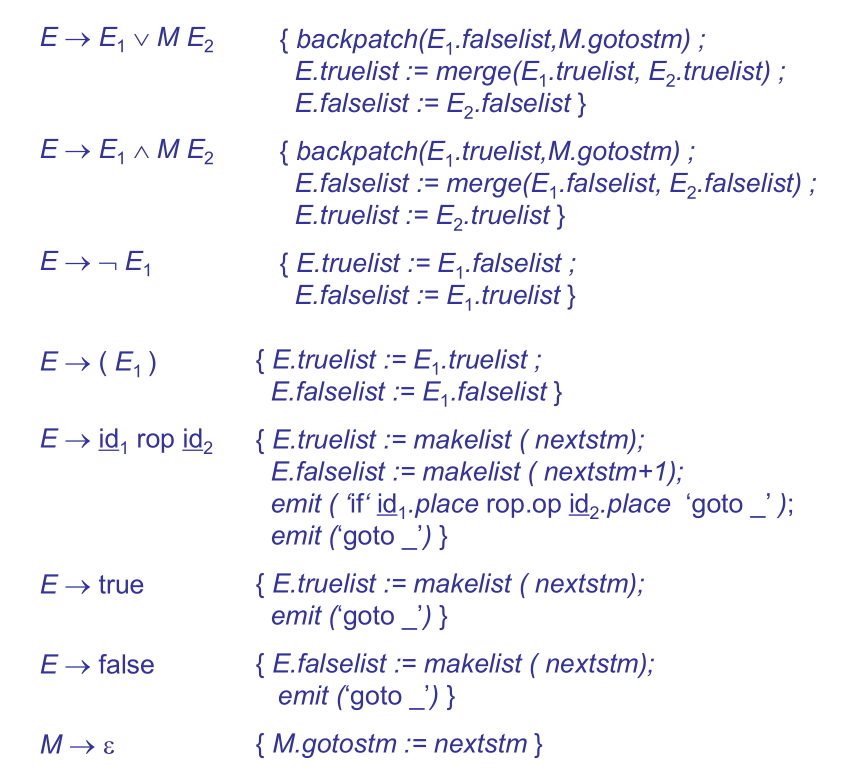
\includegraphics[width=0.9\textwidth]{bool-2.png}
    \caption{S-属性文法的布尔短路翻译}
    \label{bool-2}
    \end{figure*}

\subsubsection{控制流的翻译}
\paragraph{L-属性文法}
    如图\ref{ctrlflow-1},
    循环通过继承属性$S.next$实现, break语句通过继承属性$S.break$传递.
    \begin{figure*}[ht]
    \centering
    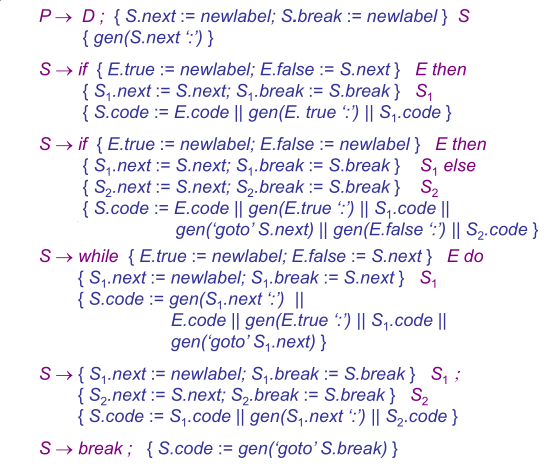
\includegraphics[width=0.9\textwidth]{ctrlflow-1.png}
    \caption{L-属性文法的控制流翻译}
    \label{ctrlflow-1}
    \end{figure*}

\paragraph{S-属性文法}
    如图\ref{ctrlflow-2},
    循环通过综合属性$S.nextlist$实现, break语句通过综合属性$S.breaklist$传递.
    \begin{figure*}[ht]
    \centering
    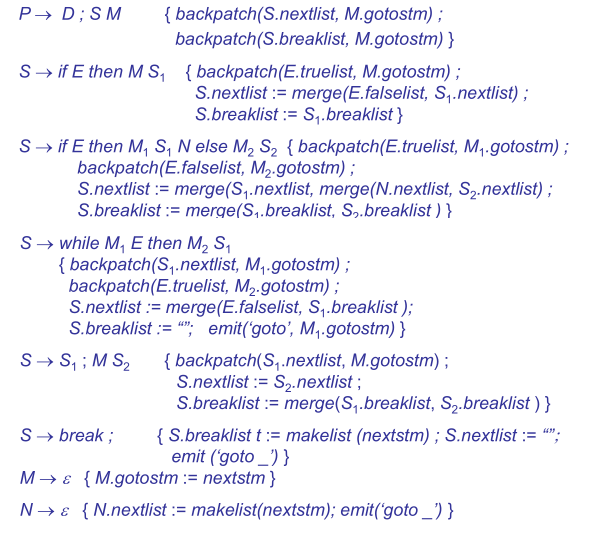
\includegraphics[width=0.9\textwidth]{ctrlflow-2.png}
    \caption{S-属性文法的控制流翻译}
    \label{ctrlflow-2}
    \end{figure*}
    \FloatBarrier

\section{运行时存储组织}
\subsection{存储分配策略}
    决定变量如何安排在内存中. 可以分为静态和动态分配, 其中动态分配又分为栈式和堆式.
\paragraph{静态分配} 
    编译期确定变量在内存中的位置, 常用于全局变量或\verb/static/变量.
    这样无法处理递归函数.
\paragraph{栈式分配}
    空间的分配根据进入退出函数在运行期确定.
    可有效实现动态嵌套的程序结构.
\paragraph{堆式分配}
    最灵活, 需要操作系统和程序员或运行时内存系统共同管理.
\subsection{活动记录}
    活动记录即栈帧, 其中保存一个函数调用的所有相关数据, 包括实参, 返回地址, 局部变量, 保存的寄存器等等.\par
\subsubsection{不允许嵌套函数}
    这种情况下, 进入一个函数分配一个栈帧, 从函数中返回就回收其 栈帧 .
    每个函数能看到的符号只有全局符号和自己栈帧中的符号.
\subsubsection{允许嵌套函数}
\paragraph{基本约定} 
    称被嵌套的函数是子函数, 嵌套其他函数的函数是父函数.
    一个子函数有且仅有一个父函数, 只有父函数的函数体中才能调用子函数.\par
    子函数能够访问父函数的变量\footnote{这里变量声明都类似Pascal语言, 是在函数体前生命的}.
\paragraph{问题}
    一个函数能看到的符号除了全局符号和自己栈帧中的符号, 还可能有父函数的符号.
    因此需要查找父函数的栈帧.
\paragraph{函数继承树}
    将所有函数按照父子函数关系建立一颗树,
    其中\verb/main/为树根, 深度为$0$.
    注意此处的\verb/main/不像C的\verb/main/是一个全局函数,
    而相当于整个程序, 可以参考Pascal的语法\begin{verbatim}program ...
... 
begin 
    (* main *) 
end;\end{verbatim} 所以全局变量是\verb/main/的变量, 全局函数是\verb/main/的子函数.\par
    容易证明, 在程序运行的任何时刻, 深度为$k$的所有函数至多有一个是活动的,
    即深度为$k$的函数至多有一个, 其栈帧在当前运行栈中.
    并且如果深度为$k$的某函数是活动的, 则一定有深度是$k-1$的某函数也是活动的, 且后者是前者的父函数.
\paragraph{Display表方法}
    维护一个表$D_n$.
    $D_n$表示从\verb/main/到当前函数在函数继承树上构成的链中,
    当前函数深度为$n$的祖先函数的栈帧位置.\par
    如对于以下程序\pagebreak
\begin{Verbatim}[samepage=true]
program main;

    function A(params): ret
        function B(params): ret
            function C(params): ret
            begin
                ... C(args); ...
            end; (* end function C *)
        begin
            ... C(args); ...
        end; (* end function B *)
    begin
        ... B(args); ...
    end; (* end function A *)

    function A1(params): ret
    begin
        ... A(args); ...
    end; (* end function A1 *)

begin
    ... A1(args); ...
end.
\end{Verbatim}
第二次运行\verb/C/时, 栈应当类似于\\
    \begin{center}\begin{tabularx}{0.6\textwidth}{r|C|c|}
        \cline{2-3}
        & whose stackframe & depth\\
        \cline{2-3}
        $D_3 \to$ & \verb/C/ & 3
        \\\cline{2-3}
        & \verb/C/ & 3
        \\\cline{2-3}
        $D_2 \to$ & \verb/B/ & 2
        \\\cline{2-3}
        $D_1 \to$ & \verb/A/ & 1
        \\\cline{2-3}
        & \verb/A1/ & 1
        \\\cline{2-3}
        $D_0 \to$ & \verb/main/ & 0
        \\\cline{2-3}
    \end{tabularx}
    \end{center}
\paragraph{维护Display}
    考虑到每次对Display表的修改至多一项,
    所以可以在栈帧中直接保存被替换的Display表项.
\paragraph{静态动态表方法}
    除了最初的\verb/main/外每个函数的栈帧都额外保存两个指针, 叫静态链和动态链.
    某函数的动态链指向本次运行中调用该函数的函数栈帧;
    静态链指向本次运行栈中其父函数, 并且是在该函数栈帧之前的第一个父函数.
\subsection{面向对象系统的实现}
\subsubsection{对象的存储组织}
\paragraph{朴素方法}
    当前对象的所有特性,
    包括继承的特性 (域和方法),
    都复制到对象存储区内.
\paragraph{类存储} 
    将每个类的结构的描述保存在类的存储空间, 使用父类指针完成继承.
    之后每个对象除了自己的成员数据外, 只需要访问自己类的结构描述得到方法.
\paragraph{虚函数表}
    将每个类的结构的描述保存在类的存储空间, 但是将父类方法也直接保存到自己类的描述.
    之后每个对象除了自己的成员数据外, 只需要访问自己类的结构描述得到方法.
    
\section{目标代码生成}
\subsection{数据流分析}
\subsubsection{概念}
    假设程序是 TAC 语句的序列. 
    \begin{description}
        \item[基本块] 如果将程序按照语句访问组织成图,
            顺序语句和无条件跳转有且只有一条出边,
            有条件跳转有两条出边.
            定义基本块是其中一条极大链, 链内部非首尾节点入度出度都为$1$.
        \item[流图] 原程序的图进行基本块缩链后, 得到的以基本块为结点的图.
            程序首条语句所在的流图结点成为流图首结点.
            一般都去掉首结点不可达的语句.
        \item[支配节点集] 流图中, 称$u$是$v$的支配节点, 
            当且仅当任何从流图首结点到$v$的路径都需要经过$u$, 记为$u \mathrm{DOM} v$
        \item[回边] 若$u \mathrm{DOM} v$且存在边$v\to u$, 则称$v\to u$是一条回边.
        \item[循环] $v\to u$是一条回边,
            则定义其对应的自然循环为
            $ \{v, u\} \cup \{ t \;|\; \exists P\;:\; t\to v, u \not\in P\} $
    \end{description}

\subsubsection{正向数据流分析}
\paragraph{定值和引用} 
    对于语句$I_n \;:\; \mathrm{lhs} = \mathrm{rhs}$,
    称$\mathrm{lhs}$中变量都被\emph{定值},
    $\mathrm{rhs}$中所有变量都被\emph{引用},
    分别记为$I_n \Def \mathrm{lhs}$,
        $I_n \Ref \mathrm{rhs}$.
    $I_n$称为$\mathrm{lhs}$的一个定值点.\par
    同一条语句中, 引用发生在定值之前.\par
    如果$I_n \Def A \;\land\; I_m \Ref A$,
    并且存在路径$P\,:\,I_n\to I_m$,
    满足$\forall I\in P\;:\; \neg(I \Def A)$,
    则称$A$的定值点$I_n$可达引用点$I_m$.
\paragraph{基本集合}
    \begin{itemize}
        \item $GEN[B]$, 是$B$中定值点的集合, 其可达$B$的出口.
        \item $KILL[B]$, 是$B$外定值点的集合, 其可达$B$的入口, 但不能达到$B$的出口.
        \item $IN[B]$, 是可达$B$入口的定值点的集合.
        \item $OUT[B]$, 是可达$B$出口的定值点的集合.
    \end{itemize}
    其中, $GEN$和$KILL$可以直接通过流图得到.
    计算时可以取$KILL$为所有可能被$B$中定值点覆盖的外部定值点.
\paragraph{到达-定值分析}
    数据流方程
    \begin{align*}
        IN[B] &= \bigcup_{C \in \mathrm{Prev}[B]} OUT[C]\\
        OUT[B] &= IN[B]\cup GEN[B] - KILL[B]
    \end{align*}
    计算集合约束问题, 即得诸集合的值.

\subsubsection{后向数据流分析}
\paragraph{活跃变量} 
    对于语句$I_n$和变量$A$, 如果存在路径$P\;:\;I_n\to I_m$,
    满足$I_m \Ref A$, 则称$A$在$I_n$处是活跃的.
\paragraph{基本集合}
    \begin{itemize}
        \item $Def[B]$, 是变量的集合, 其在$B$中被引用前被定值
        \item $LiveUse[B]$, 是变量的集合, 其在$B$中被定值前被引用
        \item $LiveIn[B]$, 是变量的集合, 其在$B$的入口寸前是活跃的
        \item $LiveOut[B]$, 是变量的集合, 其在$B$的出口寸后是活跃的
    \end{itemize}
    一定有$Def \cap LiveUse = \emptyset$
\paragraph{活跃变量分析}
    数据流方程
    \begin{align*}
        LiveOut[B] &= \bigcup_{C \in \mathrm{Succ}[B]} LiveIn[B]\\
        LiveIn[B] &= LiveOut[B] \cup LiveUse[B] - Def[B]
    \end{align*}
    计算集合约束问题, 即得诸集合的值.

\subsubsection{其他流信息}
\paragraph{UD链} 考虑$I_n$点引用了$A$的值, 则定义$A$在$I_n$的引用-定值链为
    \[\{ I \;|\; I \Def A \land I \text{可达} I_n\}\]\par
    显然, 如果$A \in Def[B]$, 那么其UD链就是$B$中定值$A$的那条语句.
    否则, 应有$A \in LiveIn[B]$, 则其UD链就是$IN[B]$中所有$A$的定值点.
\paragraph{DU链} 考虑$I_n$点定义了$A$的值, 则定义$A$在$I_n$的定值-引用链为
    \[\{ I \;|\; I \Ref A \land I_n \text{可达} I\}\]\par
\paragraph{待用信息和活跃信息}
    待用信息追踪变量在一个基本块中下一次引用的位置. 考虑加上待用信息注解,
    则需要对于基本块中每个语句其中每个变量, 找到该基本块中其下一次被引用的位置,
    然后标记在右上角标. 位置用语句的编号表示, 编号从1开始, 如果没有下一次引用则置为0.\par
    
    活跃信息追踪变量的一个值的生命周期. 考虑加上活跃信息注解,
    即对基本块中每个语句中每个变量加一个右上角标, 为L或者F.
    如果是L, 表示此变量还会在被定值前被引用;
    为F则表示此变量的这个值已经不会被引用了.
    初始条件可以从基本块的$LiveOut$信息得到.

\subsection{基本块的DAG表示}
\paragraph{约定} 基本块中, 只考虑三种语句, 如图
    \begin{figure*}[ht]
    \centering
    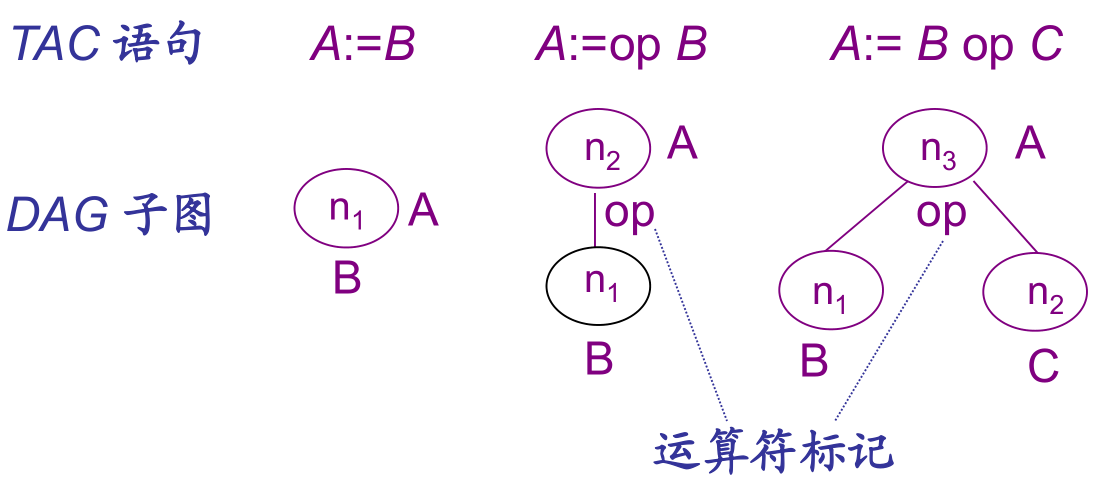
\includegraphics[width=0.9\textwidth]{bb-dag.png}
    \caption{三种语句, 以及其DAG子图表示}
    \label{bb-dag}
    \end{figure*}
    之后, 对于每一个语句. 如果其$\mathrm{rhs}$中, 
    有变量没有对应的结点, 则为其新建一个结点.\par
    之后构建过程中, 完成的优化有合并常量,
    删除冗余运算, 合并已知量, 删除无用赋值.
    例如下图.
    \begin{figure*}[ht]
    \centering
    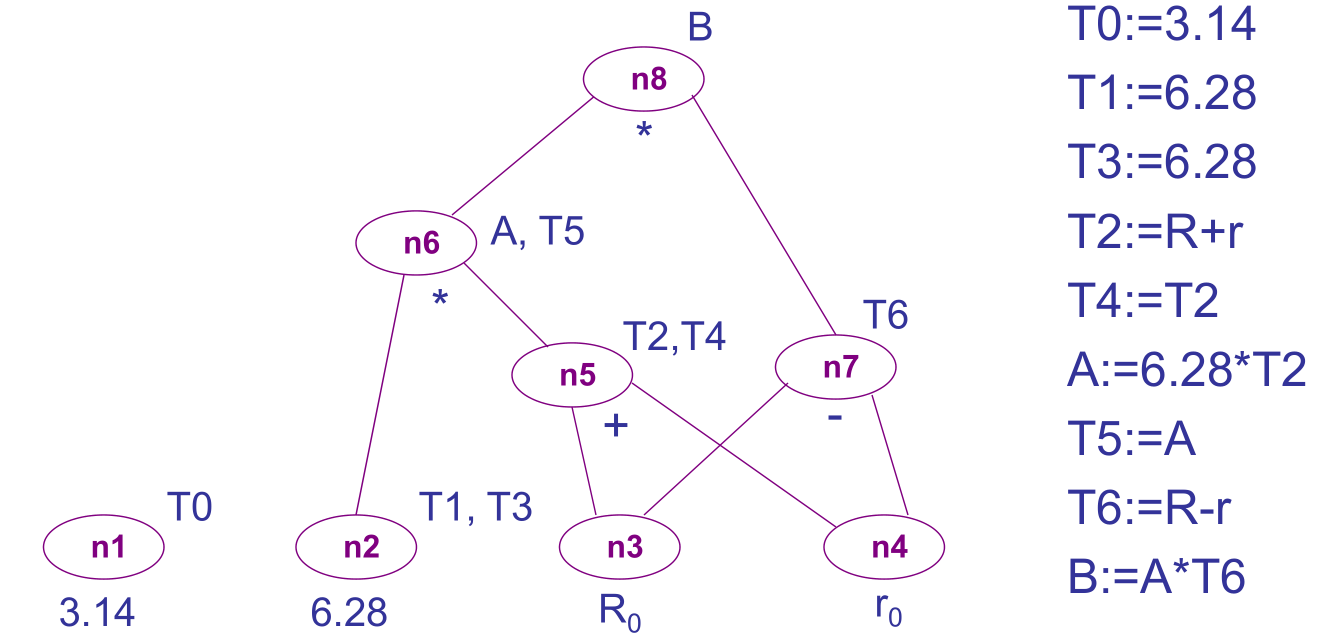
\includegraphics[width=0.9\textwidth]{bb-dag-ex.png}
    \caption{右边的基本块生成左边的DAG}
    \label{bb-dag-ex}
    \end{figure*}

\subsection{代码生成}
\subsubsection{指令选择}
\paragraph{要求} 首先要求正确性, 即意思不改变.
    其次是代价, 包括减少语句条数, 减少内存访问等等.
    具体实现通过AVALUE和RVALUE来完成, 即及时维护一个寄存器-变量的一对多关系.
\subsubsection{Ershov数} 一个表达式的Ershov数定义为其求值所需最少多少寄存器.\par
    可以递归地计算, 考虑表达式树(DAG亦可)$T$, 左右儿子是$L$, $R$. 有\[
        \text{Ershov}(T) = \begin{cases}
            1 & L = R = \text{NULL}\\
            \text{Ershov}(R) & L = \text{NULL}\\
            \text{Ershov}(L) & R = \text{NULL}\\
            \text{Ershov}(L) + 1 & \text{Ershov}(L) = \text{Ershov}(R)\\
            max\{\text{Ershov}(L), \text{Ershov}(R)\} & \text{Ershov}(L) \neq \text{Ershov}(R)\\
        \end{cases}\]
    由Ershov数的定义容易得到求值算法 (Sethi-Ullman算法)
\subsubsection{寄存器分配}
    即将伪寄存器映射到物理寄存器的方法, 不考虑到泄露到内存的情况.
    采用寄存器相干图. 原理是, 如果在$A$的定值点寸后$B$是活跃的,
    则$A$, $B$应当分配到不同的物理存储器. 于是将伪寄存器作为结点建图,
    求图色数就是程序最少使用的物理存储器.

%\paragraph{程序内存布局} 程序的虚拟内存空间的典型安排如\\
%    \begin{center}
%    \begin{tabularx}{0.5\textwidth}{|C|}
%        \hline
%        0xFFFF\ldots\\
%        \hline
%        保留\\
%        \hline
%        栈\\
%        $\downarrow$\\
%        \hline
%        $\uparrow$\\
%        堆\\
%        \hline
%        运行时库\\
%        \hline
%        静态数据\\
%        \hline
%        代码段\\
%        \hline
%        保留\\
%        \hline
%        0x0000\ldots\\
%        \hline
%    \end{tabularx}
%    \end{center}

%If the attributes are all synthesized, and the actions occur at the ends of the
%productions, then we can compute the attributes for the head when we reduce
%the body to the head
\end{document}
